\section{Experimental Evaluation}

\subsection{Experimental setup} \label{subsec:setup}

Our data set consists of 148 process descriptions annotated by a biologist. The annotator was presented with annotation guidelines, annotated 20 descriptions and then annotations were discussed with the authors, after which all process descriptions were annotated. After training a second biologist, we measured inter-annotator agreement on 30 random process descriptions, resulting in agreement $\kappa=0.69$. 

Process descriptions were parsed with Stanford constituency and dependency parsers \cite{Klein03,Marneffe06}, and 35 process descriptions were set aside as a test set (\# of training set trigger pairs: 1932, \# of test set trigger pairs: 906). We performed 10-fold cross validation over the training set for feature selection and tuning of constraint parameters. For each constraint type (connectivity, chain-structure, and five triangle constraints) we introduced a parameter and tuned the seven parameters by coordinate-wise ascent, where for hard constraints a binary parameter controls whether the constraint is used, and for soft constraints we attempted 10 different reward/penalty values. Last, for our global model we defined $\theta_{ijr}=\log p_{ijr}$, where $p_{ijr}$ is the probability given by the local classifier.

We test the following systems: (a) \emph{All-Prev}: since the most common process structure is a chain of consecutive events we simply predict \textsc{Next} for every two adjacent triggers. (b) \emph{Local$_{base}$}: A pairwise classifier with features from previous work (Section~\ref{subsec:pairwise}) (c) \emph{Local} A pairwise classifier with all features (Section~\ref{subsec:pairwise-novel}) (d) \emph{Global}: Our full model that uses ILP inference.

%(d) \emph{Local$_{chain}$}: For every two adjacent triggers we pick the highest probability non-\textsc{None} relation using the local classifier. Again, this uses the assumption that many processes have a chain-structure.

To evaluate system performance we compare the set of predictions on all trigger pairs to the gold standard annotations and compute micro-averaged precision, recall and F$_1$. We perform two types of evaluations: (a) \emph{Full}: evaluation on our full set of 11 relations (b) \emph{Temporal:} Evaluation on temporal relations only, by collapsing \textsc{Prev}, \textsc{Causes}, and \textsc{Enables} to a single category and similarly for \textsc{Next}, \textsc{Caused}, and \textsc{Enabled} (inter-annotator agreement $\kappa=0.75$). We computed statistical significance of our results with the paired bootstrap resampling method \cite{efron1993}.

\subsection{Results} \label{subsec:results}

\begin{table}[t]
{\footnotesize
\begin{tabular}{| l | c | c | c | c | c | c |}
\hline
    & \multicolumn{3}{c|}{\textbf{Temporal}} & \multicolumn{3}{c|}{\textbf{Full}} \\
    & P & R & F$_1$ & P & R & F$_1$ \\
\hline
\hline
\emph{All-Prev} & 62.2 & 58.3 & 60.2 & 34.1 & 32.0 & 33.0 \\
%\emph{Local$_{base}$} & 65.7 & 49.6 & 56.5 &  51.7 & 39.0 & 44.5\\
\emph{Local$_{base}$} & 65.6 & 55.3 & 60.0 &  52.1 & 43.9 & 47.6\\
\emph{Local} & 66.2 & 58.3 & 62.0 & 54.7 & 48.3 & 51.3 \\
%\emph{Local} & 50.3 & \textbf{67.8} & 52.6 & 59.3 & \textbf{57.6} & 44.7 \\
%\emph{Local$_{chain}$} & 65.0 & 60.1 & 62.9 & 52.8 & 49.6  & 51.1 \\
\emph{Global} & \textbf{67.1} & \textbf{64.5*} & \textbf{65.8*} & \textbf{56.2} & \textbf{54.0*} & \textbf{55.0*} \\
\hline
\end{tabular}}
\caption{Test set results on all experiments. Asterisk (*) denotes statistical significance ($p<0.01$) against all other baselines. \textcolor{red}{TODO} compute stat significant for real}
\label{tab:results}
\end{table}

Table~\ref{tab:results} presents performance of all systems. Our main result is that using global constraints improves performance on all measures in both full and temporal evaluations. Particularly, in the full evaluation recall improves by 12\% and overall F$_1$ improves significantly by 3.7 points against \emph{Local} ($p<0.01$). Recall improvement suggests that modeling connectivity allowed \emph{Global} to add correct relations in cases where some events were not connected to one another.

The full \emph{Local} classifier substantially outperforms \emph{Local$_{base}$}. This indicates that our novel features (Section~\ref{subsec:pairwise-novel}) are important for discriminating between process relations. Specifically, in the full evaluation \emph{Local} improves precision more than in the temporal evaluation, suggesting that designing syntactic and semantic features for connectives is useful for distinguishing \textsc{Next}, \textsc{Causes}, and \textsc{Enables} when the amount of training data is small.

The \emph{All-Prev} baseline performs quite badly in the full evaluation, but in temporal evaluation it performs reasonably well. This demonstrates the strong tendency process descriptions have to proceed linearly from one event to the other, which is a general property of discourse structure \cite{schegloff73}.

Table~\ref{tab:degree} presents the degree distribution of \emph{Local} and \emph{Global} on the development set comparing to the gold standard. Clearly, degree distribution of \emph{Global} is much more similar to the gold standard than \emph{Local}. In particular, the connectivity constraint ensures that there are no isolated nodes and shifts mass from nodes with degree $0$ and $1$ to nodes with degree $2$.

Table~\ref{tab:paramtuning} presents the order in which global constraints were introduced into the model using coordinate ascent on the development set. Connectivity is the first constraint to be introduced, and improves performance considerably. The chain constraint, on the other hand, is included third, which can be explained by examining the distribution of degrees in Table~\ref{tab:degree}. The predictions of \emph{Local} do not have many nodes with degree $>2$ and thus the effect of this constraint is smaller. As for triangle constraints, we see that four constraints are included in the model but one is discarded since it did not improve F$_1$ on the development set.

\begin{table}[t]
{\footnotesize
\begin{tabular}{| l | c | c | c |}
\hline
    \textbf{Order} & \textbf{Parameter name} & \textbf{Value} ($\alpha$)& \textbf{F$_1$ score} \\
\hline
\hline
- & \emph{Local model} & - & 49.9 \\
1 & Connectivity constraint & $\infty$ & 51.2 \\
2 & \textsc{Same} transitivity &  0.5 & 52.9 \\
3 & Chain constraint & -0.5 & 53.3\\
4 & \textsc{Cause}-\textsc{Cotemp} & 1.0 & 53.7\\
6 & \textsc{Prev} contradiction & $\infty$ & 53.8\\
7 & \textsc{Same} contradiction & $\infty$ & 53.9\\

\hline
\end{tabular}}
\caption{Order by which constraint parameters were set using coordinate ascent on the development set. For each parameter, the value chosen and F$_1$ score after including the constraint are provided. Negative values correspond to penalties, positive values to rewards, and a value of $\infty$ indicates a hard constraint.}
\label{tab:paramtuning}
\end{table}

\subsection{Qualitative Analysis} \label{subsec:analysis}

\begin{figure*}[t]
\centering
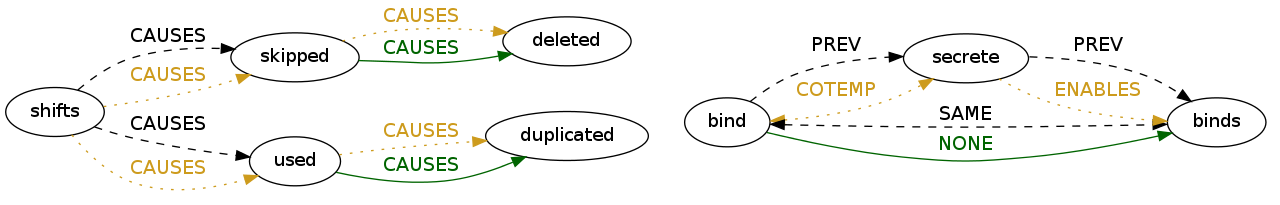
\includegraphics[width=0.99\textwidth]{figures/example.png} 
\caption{Fragments of process graphs. Black edges are predictions of \emph{Local}, green edges indicate edges modified by \emph{Global}, and gold edges represent gold standard edges. Original text, Left: ``... the template \emph{shifts} with respect to the new complementary strand, and a part of the template strand is either \emph{skipped} by the replication machinery or \emph{used} twice as a template.
As a result, a segment of DNA is \emph{deleted} or \emph{duplicated}." Right: ``Cells of mating type A secrete a signaling molecule, which can \emph{bind} to specific receptor proteins on nearby cells. At the same time, cells \emph{secrete} factor, which \emph{binds} to receptors on a cells."}
\label{fig:graph}
\end{figure*}

Figure~\ref{fig:graph} shows two examples where global constraints corrected predictions made by \emph{Local}. In Figure~\ref{fig:graph}, left, \emph{Local} failed to predict the causal relations \emph{skipped}-\emph{deleted} and \emph{used}-\emph{duplicated}, possibly because they are not in the same sentence and are not adjacent to one another. By enforcing a connectivity constraint, \emph{Global} was able to connect the triggers \emph{deleted} and \emph{duplicated} to the other triggers in the process using the correct relations.

In Figure~\ref{fig:graph}, right, \emph{Local} predicts a triangle that violates the ``\textsc{Same} contradiction" constraint. The triggers \emph{bind} and \emph{binds} cannot denote the same event if a third trigger \emph{secrete} is temporally between them. However, since \emph{bind} and \emph{binds} share the same lemma, \emph{Local} predicts that they are co-referring triggers. Global constraints prohibit this solution and as a result \emph{Global} modifies the solution and correctly predicts \textsc{None}.

In general, the local model learns feature weights that favor the more dominant classes - \textsc{Prev} and \textsc{Causes}, which generally happens with classifiers trying to maximize the overall score. In addition, the relation types \textsc{Causes} and \textsc{Enables} are harder to differentiate from \textsc{Prev} as demonstrated in Figure~\ref{fig:graph} right. This is expected as temporally, all three relations mean the same, but have very subtle differences. With some of the examples, even human annotators find it hard to differentiate between the three classes. Analyzing the confusion matrix of the predictions also gave several insights:
\begin{enumerate}
\item The mass is concentrated across the diagonal.
\item The class-specific F1 score reduces with how prevalent the class is.
\item The most common misclassification is between PREV-CAUSES and PREV-COTEMP.
\end{enumerate}
